\documentclass[10pt,t]{beamer}
\usepackage[utf8]{inputenc}
\usepackage[T1]{fontenc}
\fontfamily{ppl}\selectfont

\usepackage{fontspec} 
\defaultfontfeatures{Mapping=tex-text} 
\setsansfont[Ligatures={Common}]{Futura}
\setmonofont[Scale=0.8]{Monaco} 


%\setbeamersize{text margin left=10pt,text margin right=10pt}
\usetheme{lehigh}

\usefonttheme{professionalfonts}
\usefonttheme{serif}

\pgfdeclarelayer{background}
\pgfdeclarelayer{foreground}
\pgfsetlayers{background,main,foreground}

% add packages to use
%\usepackage[latin1]{inputenc}
%\usepackage[english]{babel}
%\usepackage[normalem]{ulem}
\usepackage{times}
\usepackage[T1]{fontenc}
\usepackage{pgf,pgfarrows,pgfnodes,pgfautomata,pgfheaps,pgfshade}
\usepackage{amsmath,amssymb,amsfonts,subfigure,pifont}
\usepackage{graphicx}
\usepackage{multirow,multicol}
\usepackage{tabularx}
\usepackage{booktabs}
\usepackage{colortbl}
\usepackage{fancyvrb,listings}
\usepackage{algorithm,algpseudocode}
%\usepackage{keystroke}
\usepackage{etex}
\usepackage{hyperref}
\usepackage{tikz}
\usetikzlibrary{trees,matrix,shapes,arrows}
\usetikzlibrary{calc}



% The following color are for listing environment 
\definecolor{dkgreen}{rgb}{0,0.6,0}
\definecolor{DarkGreen}{rgb}{0.0,0.3,0.0}
\definecolor{gray}{rgb}{0.5,0.5,0.5}
\definecolor{mauve}{rgb}{0.58,0,0.82}
\definecolor{Blue}{rgb}{0.0,0.0,0.8} 
\definecolor{dodgerblue}{rgb}{0.1,0.1,1.0}
\definecolor{indigo}{rgb}{0.41,0.1,0.0}
\definecolor{seagreen}{rgb}{0.1,1.0,0.1}


\lstset{%
language=bash,                % the language of the code
basicstyle=\tiny\ttfamily,           % the size of the fonts that are used for the code
showspaces=false,               % show spaces adding particular underscores
showstringspaces=false,         % underline spaces within strings
showtabs=false,                 % show tabs within strings adding particular underscores
%frame=single,                   % adds a frame around the code
%rulecolor=\color{black},        % if not set, the frame-color may be changed on line-breaks within not-black text (e.g. comments (green here))
tabsize=2,                      % sets default tabsize to 2 spaces
%captionpos=b,                   % sets the caption-position to bottom
breaklines=true,                % sets automatic line breaking
breakatwhitespace=false,        % sets if automatic breaks should only happen at whitespace
%title=\lstname,                   % show the filename of files included with \lstinputlisting;
% also try caption instead of title
keywordstyle=\color{blue},          % keyword style
commentstyle=\color{dkgreen},       % comment style
stringstyle=\color{mauve},         % string literal style
escapeinside={!}{!},            % if you want to add LaTeX within your code
morekeywords={*,\dots,elif},              % if you want to add more keywords to the set
deletekeywords={\dots},              % if you want to delete keywords from the given language
%morecomment=[l]{//}
}
\lstset{%
language=csh,                % the language of the code
basicstyle=\tiny\ttfamily,           % the size of the fonts that are used for the code
showspaces=false,               % show spaces adding particular underscores
showstringspaces=false,         % underline spaces within strings
showtabs=false,                 % show tabs within strings adding particular underscores
%frame=single,                   % adds a frame around the code
%rulecolor=\color{black},        % if not set, the frame-color may be changed on line-breaks within not-black text (e.g. comments (green here))
tabsize=2,                      % sets default tabsize to 2 spaces
captionpos=b,                   % sets the caption-position to bottom
breaklines=true,                % sets automatic line breaking
breakatwhitespace=false,        % sets if automatic breaks should only happen at whitespace
%title=\lstname,                   % show the filename of files included with \lstinputlisting;
% also try caption instead of title
keywordstyle=\color{blue},          % keyword style
commentstyle=\color{dkgreen},       % comment style
stringstyle=\color{mauve},         % string literal style
escapeinside={\%*}{*)},            % if you want to add LaTeX within your code
morekeywords={*,\dots,elif},              % if you want to add more keywords to the set
deletekeywords={\dots},              % if you want to delete keywords from the given language
%morecomment=[l]{//}
}

\lstdefinestyle{LINUX}
{
    backgroundcolor=\color{white},
    basicstyle=\tiny\ttfamily,
    keywordstyle=\color{blue},
    morekeywords={apacheco,Tutorials,BASH,scripts,day1,examples},
    literate={>}{{\textcolor{blue}{>}}}1
         {/}{{\textcolor{blue}{/}}}1
         {./}{{\textcolor{black}{./ }}}1
         {~}{{\textcolor{blue}{\textasciitilde}}}1,
}

\lstdefinestyle{customc}{
  belowcaptionskip=1\baselineskip,
  breaklines=true,
  xleftmargin=\parindent,
  language=C,
  showstringspaces=false,
  basicstyle=\tiny\ttfamily,
  keywordstyle=\bfseries\color{green!40!black},
  commentstyle=\upshape\color{red!90!white},
  identifierstyle=\color{blue},
  stringstyle=\color{orange},
}
\lstdefinelanguage{OmpFortran}[]{Fortran}{
   rulesepcolor=\color{black},
   %
   extendedchars=true,
   %
   morecomment=[l] [\bfseries\color{red!90!white}]{!\$omp},
   morecomment=[l] [\bfseries\color{red!90!white}]{c\$omp},
   morecomment=[l] [\bfseries\color{red!90!white}]{*\$omp},
   morecomment=[l] [\bfseries\color{red!90!white}]{!\$acc},
   morecomment=[l] [\bfseries\color{red!90!white}]{c\$acc},
   morecomment=[l] [\bfseries\color{red!90!white}]{*\$acc},
}[comments]

\lstdefinelanguage{OmpC}[]{OmpFortran}{
   rulesepcolor=\color{black},
   %
   extendedchars=true,
   %
   morecomment=[l] [\bfseries\color{red!90!white}]{\#pragma\ omp},
   morecomment=[l] [\bfseries\color{red!90!white}]{\#pragma\ acc},
}[comments]

\lstset{escapechar=@,style=customc}
\lstset{literate=%
   *{0}{{{\color{blue}0}}}1
    {1}{{{\color{blue}1}}}1
    {2}{{{\color{blue}2}}}1
    {3}{{{\color{blue}3}}}1
    {4}{{{\color{blue}4}}}1
    {5}{{{\color{blue}5}}}1
    {6}{{{\color{blue}6}}}1
    {7}{{{\color{blue}7}}}1
    {8}{{{\color{blue}8}}}1
    {9}{{{\color{blue}9}}}1
}

\algrenewcommand\algorithmicfunction{\textbf{program}}
\algblockdefx[Program]{Program}{EndProgram}[1]{\textbf{program} \textsc{#1}}[1]{\textbf{end program} \textsc{#1}}
\algloopdefx[doloop]{Do}[1]{\textbf{do} #1}
\algcblockdefx[doloop]{If}{Do}{EndDo}
[1]{\textbf{do} #1}{\textbf{end do}}


\DeclareSymbolFont{extraup}{U}{zavm}{m}{n}
%\DeclareMathSymbol{\vardiamond}{\mathalpha}{extraup}{87}
\newcommand{\cmark}{\ding{51}}
\newcommand{\xmark}{\ding{55}}
\newcommand{\smark}{\ding{77}}
\newcommand*\vardiamond{\textcolor{lubrown}{%
  \ensuremath{\blacklozenge}}}
\newcommand*\mybigstar{\textcolor{lubrown!90!yellow}{%
  \ensuremath{\bigstar}}}
\newcommand*\up{\textcolor{green!80!black}{%
  \ensuremath{\blacktriangle}}}
\newcommand*\down{\textcolor{red}{%
  \ensuremath{\blacktriangledown}}}
\newcommand*\const{\textcolor{darkgray}%
  {\textbf{--}}}
\newcommand*\enter{\tikz[baseline=-0.5ex] \draw[<-] (0,0) -| (0.5,0.1);}
\newcommand{\bftt}[1]{\textbf{\texttt{#1}}}
\newcommand{\bflub}[1]{\textbf{\color{lubrown}#1}}
\newcommand{\lstfortran}[1]{\lstinline[language={[90]Fortran},basicstyle=\small\ttfamily]|#1|}
\newcommand{\lstC}[1]{\lstinline[language=C,basicstyle=\small\ttfamily]|#1|}
\newcommand{\Verblubrown}[1]{\Verb[formatcom=\color{lubrown},fontseries=b,commandchars=\\\{\}]|#1|}
\newcommand{\Verblue}[1]{\Verb[formatcom=\color{lublue},fontseries=b,commandchars=\\\{\}]!#1!}
\newcommand{\Verbblue}[2][b]{\Verb[formatcom=\color{lublue},fontshape=#1,commandchars=\\\{\}]|#2|}
\newcommand{\Verblubrownp}[1]{\Verb[formatcom=\color{lubrown},fontseries=b,commandchars=\\\{\}]!#1!}
\newcommand{\Verbred}[1]{\Verb[formatcom=\color{red},commandchars=\\\{\}]|#1|}
\newcommand{\Verbindigo}[1]{\Verb[formatcom=\color{indigo},fontsize=\fontsize{7.5}{8}\selectfont,commandchars=\\\{\}]!#1!}

\newcolumntype{a}{>{\columncolor{lulime}}c}
\newcolumntype{b}{>{\columncolor{lulime!50}}c}
\newcolumntype{d}{>{\columncolor{lulime!40}}c}
\newcolumntype{e}{>{\columncolor{lulime}}l}
\newcolumntype{f}{>{\columncolor{lulime!50}}l}

                           
% LOGOS
\pgfdeclareimage[height=0.55cm]{lucolor-logo}{LehighU_official-logo_Color.png}
\rplogo{\pgfuseimage{lucolor-logo}}
\pgfdeclareimage[height=0.55cm]{luwhite-logo}{LehighU_official-logo_White.png}
\tplogo{\pgfuseimage{luwhite-logo}}
% footer logo
%\pgfdeclareimage[width=0.3\paperwidth]{university-logo}{lulogo}
%\tllogo{\pgfuseimage{university-logo}}

%titlepage logo
%\titlegraphic{
\includegraphics[scale=0.5]{lu}}

\beamertemplateballitem



\title{Introduction to OpenACC}
\subtitle{2021~HPC~Workshop:~Parallel~Programming}
\author{\large{Alexander~B.~Pacheco}}
\institute[Lehigh University Research Computing]{\href{http://researchcomputing.lehigh.edu}{Research~Computing}}
\date{July~13~-~15,~2021}
    

\begin{document}

\begin{frame}
  \titlepage
\end{frame}

\begin{frame}{CPU vs GPU}
  \begin{description}
    \item[CPU]: consists of a few cores optimized for sequential serial processing
    \item[GPU]: has a massively parallel architecture consisting of thousands of smaller, more efficient cores designed for handling multiple tasks simultaneously
    \item[] \href{http://www.nvidia.com/object/gpu-applications.html}{GPU enabled applications}
  \end{description}
  \centering{
    \only<1>{\includegraphics[width=0.5\textwidth]{./cpu-and-gpu} }
    \only<2>{\includegraphics[width=0.75\textwidth]{./gpu-devotes-more-transistors-to-data-processing} }
    \only<3>{\includegraphics[width=0.75\textwidth]{./floating-point-operations-per-second} }
    \only<4>{\includegraphics[width=0.5\textwidth]{./memory-bandwidth} }
    }
\end{frame}

\begin{frame}{GPU Design}
  \vspace{0.25cm}
  \begin{center}
    \includegraphics[width=0.8\textwidth]{./Slide03}
  \end{center}
\end{frame}

\begin{frame}{Hetergenous Programming}
  \begin{center}
    \includegraphics[width=\textwidth]{./application_code}
  \end{center}
\end{frame}

\begin{frame}{Accelerate Application for GPU}
  \begin{center}
    \includegraphics[width=\textwidth]{./gpuaccelerateapp}
  \end{center}
\end{frame}

\begin{frame}{GPU Accelerated Libraries}
  \begin{center}
    \includegraphics[width=\textwidth]{./gpuacceleratedapps}
  \end{center}
\end{frame}

\begin{frame}{GPU Programming Languages}
  \begin{center}
    \includegraphics[width=\textwidth]{./gpuproglang}
  \end{center}
\end{frame}

\begin{frame}{Accelerator Fundamentals}
  \begin{itemize}
    \item We must expose enough parallelism to saturate the device
      \begin{itemize}
        \item Accelerator threads are slower than CPU threads
        \item Accelerators have orders of magnitude more threads
      \end{itemize}
    \item Fine grained parallelism is good
    \item Coarse grained parallelism is bad
      \begin{itemize}
        \item Lots of legacy apps have only exposed coarse grain parallelism
          \begin{itemize}
            \item i.e. MPI and possibly OpenMP
          \end{itemize}
      \end{itemize}
  \end{itemize}
\end{frame}

\begin{frame}[allowframebreaks]{What is OpenACC?}
  \begin{columns}
  \column{0.5\textwidth}
  \begin{center}
    \includegraphics[width=\textwidth]{./whatisopenacc}
  \end{center}
  \column{0.5\textwidth}
  \begin{block}{}
    \begin{itemize}
      \item Open Standard
      \item Easy, Compiler-Driven Approach
      \item portable across host CPUs and accelerators
      %\item OpenACC Application Program Interface describes a collection of compiler directive to specify loops and regions of code in standard C, C++ and Fortran to be offloaded from a host CPU to an attached accelerator.
      %\item provides portability across operating systems, host CPUs and accelerators
    \end{itemize}
  \end{block}
  \end{columns}	

  \framebreak

  \begin{exampleblock}{History}
    \begin{itemize}
    \item OpenACC was developed by The Portland Group (PGI), Cray, CAPS and NVIDIA. 
    \item PGI, Cray, and CAPs have spent over 2 years developing and shipping commercial compilers that use directives to enable GPU acceleration as core technology. 
    \item The small differences between their approaches allowed the formation of a group to standardize a single directives approach for accelerators and CPUs.
    \item Full OpenACC 2.0 Specification available online 
      \begin{itemize}
      \item \url{http://www.openacc-standard.org/}
      \item Implementations available now from PGI and Cray
      \end{itemize}
    \end{itemize}
  \end{exampleblock}

  \begin{exampleblock}{The Standard for GPU Directives}
    \begin{description}
      \item[Simple:] Directive are the easy path to accelerate compute intensive applications
      \item[Open:] OpenACC is an open GPU directives standard, making GPU programming straightforwards and portable across parallel and multi-core processors
      \item[Powerful:] GPU directives allow complete access to the massive parallel power of a GPU
    \end{description}
  \end{exampleblock}
\end{frame}

\begin{frame}{What is OpenACC?}
  \vspace{-0.5cm}
  \begin{exampleblock}{High Level}
    \begin{itemize}
      \item Compiler directives to specify parallel regions in C \& Fortran
      \begin{itemize}
        \item Offload parallel regions
        \item Portable across OSes, host CPUs, accelerators, and compilers
      \end{itemize}
      \item Create high-level heterogenous programs
      \begin{itemize}
        \item Without explicit accelerator intialization
        \item Without explicit data or program transfers between host and accelerator
      \end{itemize}
    \end{itemize}
  \end{exampleblock}
  \begin{exampleblock}{High Level $\cdots$ with low-level access}
    \begin{itemize}
      \item Programming model allows programmers to start simple
      \item Compiler gives additional guidance
      \begin{itemize}
        \item Loop mappings, data location and other performance details
      \end{itemize}
      \item Compatible with other GPU languages and libraries
      \begin{itemize}
        \item Interoperate between CUDA C/Fortran and GPU libraries
        \item e.g. CUFFT, CUBLAS, CUSPARSE, etc
      \end{itemize}
    \end{itemize}
  \end{exampleblock}
\end{frame}

\begin{frame}{ Why OpenACC}
  \begin{exampleblock}{}
    \begin{itemize}
      \item Directives are easy and powerful.
      \item Avoid restructuring of existing code for production applications.
      \item Focus on expressing parallelism.
    \end{itemize}
  \end{exampleblock}
  \vspace{1cm}
  \begin{alertblock}{}
    \begin{center}
      \vspace{0.1cm}
      \Large{\color{red!80!black}OpenACC is not GPU Programming}\\
      \vspace{1cm}
      \Large{\color{red!80!black}OpenACC is Expressing Parallelism in your code}
    \end{center}
  \end{alertblock}
\end{frame}

\begin{frame}{ OpenACC Execution Model}
  \begin{exampleblock}{}
    \begin{itemize}
      \item Application code runs on the CPU (sequential, shared or distributed memory)
      \item OpenACC directives indicate that the following block of compute intensive code needs to be offloaded to the GPU or accelerator.
    \end{itemize}
    \vspace{-0.5cm}
        \begin{center}
      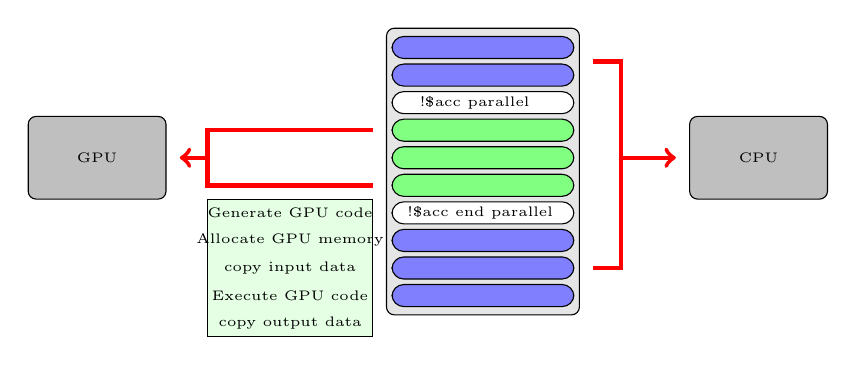
\begin{tikzpicture}[scale=0.35]
        \tikzstyle{every node}=[font=\tiny]
        \filldraw[fill=gray!20!white,rounded corners=1mm] (0,-0.2) rectangle (7,10.2);
        \filldraw[fill=blue!50!white,rounded corners=1.5mm] (0.2,0.1) rectangle (6.8,0.9);
        \filldraw[fill=blue!50!white,rounded corners=1.5mm] (0.2,1.1) rectangle (6.8,1.9);
        \filldraw[fill=blue!50!white,rounded corners=1.5mm] (0.2,2.1) rectangle (6.8,2.9);
        \filldraw[fill=white,rounded corners=1.5mm] (0.2,3.1) rectangle (6.8,3.9);
        \filldraw[fill=green!50!white,rounded corners=1.5mm] (0.2,4.1) rectangle (6.8,4.9);
        \filldraw[fill=green!50!white,rounded corners=1.5mm] (0.2,5.1) rectangle (6.8,5.9);
        \filldraw[fill=green!50!white,rounded corners=1.5mm] (0.2,6.1) rectangle (6.8,6.9);
        \filldraw[fill=white,rounded corners=1.5mm] (0.2,7.1) rectangle (6.8,7.9);
        \filldraw[fill=blue!50!white,rounded corners=1.5mm] (0.2,8.1) rectangle (6.8,8.9);
        \filldraw[fill=blue!50!white,rounded corners=1.5mm] (0.2,9.1) rectangle (6.8,9.9);
        \draw (3.4,3.5) node {!\$acc end parallel};
        \draw (3.2,7.5) node {!\$acc parallel};
        \draw[ultra thick,red] (7.5,1.5) -- (8.5,1.5) -- (8.5,9.0) -- (7.5,9.0);
        \draw[->,ultra thick,red] (8.5,5.5) -- (10.5,5.5);
        \draw[ultra thick,red] (-0.5,4.5) -- (-6.5,4.5) -- (-6.5,6.5) -- (-0.5,6.5);
        \draw[->,ultra thick,red] (-6.5,5.5) -- (-7.5,5.5);
        \filldraw[fill=gray!50!white,rounded corners=1mm] (-8.0,4.0) rectangle (-13.0,7,0);
        \filldraw[fill=gray!50!white,rounded corners=1mm] (11.0,4.0) rectangle (16.0,7,0);
        \draw (-10.5,5.5) node {GPU};
        \draw (13.5,5.5) node {CPU};
        \filldraw[fill=green!10!white] (-6.5,-1.0) rectangle (-0.5,4.0);
        \draw (-3.5,3.5) node {Generate GPU code};
        \draw (-3.5,2.5) node {Allocate GPU memory};
        \draw (-3.5,1.5) node {copy input data};
        \draw (-3.5,0.5) node {Execute GPU code};
        \draw (-3.5,-0.5) node {copy output data};
      \end{tikzpicture}
      \vspace{-0.8cm}
    \end{center}

  \end{exampleblock}
\end{frame}

\begin{frame}[fragile]{OpenACC Directive Syntax}
  \begin{exampleblock}{C/C++}
    \lstinline[basicstyle=\fontsize{12}{14}\selectfont,language=OmpC]|#pragma acc directive [clause [,] clause] ...]|
\\
     ... often followed by a structured code block
  \end{exampleblock}

  \begin{exampleblock}{Fortran}
    \lstinline[basicstyle=\fontsize{12}{14}\selectfont,language=OmpFortran]|!$acc directive [clause [,] clause] ...]|
      \\
      ...often paired with a matching end directive surrounding a structured  code block:
      \\
      \lstinline[basicstyle=\fontsize{12}{14}\selectfont,language=OmpFortran]|!$acc end directive|
  \end{exampleblock}
\end{frame}

\begin{frame}[fragile,c]{OpenACC kernels directive}
  \begin{itemize}
  \item[C:] \Verbred{\#pragma acc kernels [clause]}
  \item[Fortran] \Verbred{!\$acc kernels [clause]}
  \item The kernels directive expresses that a region may contain parallelism and the compiler determines what can be safely parallelized.
  \item The compiler breaks code in the kernel region into a sequence of kernels for execution on the accelerator device.
  \item {\color{red}What is a kernel?} {\color{DarkGreen}A function that runs in parallel on the GPU.}
  \item When a program encounters a kernels contruct, it will launch a sequence of kernels in order on the device.
  \end{itemize}
  \vspace{-0.5cm}
  \begin{columns}
    \column{0.45\textwidth}
    \begin{exampleblock}{Fortran}
      \lstinputlisting[basicstyle=\tiny\ttfamily,language=OmpFortran,firstline=98,lastline=107]{src/tmp.f90}
    \end{exampleblock}
    \column{0.45\textwidth}
    \begin{exampleblock}{C/C++}
      \lstinputlisting[basicstyle=\tiny\ttfamily,language=OmpC,firstline=50,lastline=60]{src/tmp.c}
    \end{exampleblock}
  \end{columns}
\end{frame}

\begin{frame}[fragile,c]{OpenACC Parallel Directive}
  \begin{itemize}
  \item The {\bf parallel} directive identifies a block of code as having parallelism.
  \item Compiler generates a parallel kernel for that loop.
  \item[C:] \Verbred{\#pragma acc parallel [clauses]}
  \item[Fortran:] \Verbred{!\$acc parallel [clauses]}
  \end{itemize}
  \vspace{-0.5cm}
  \begin{columns}
    \column{0.45\textwidth}
    \begin{exampleblock}{Fortran}
      \lstinputlisting[basicstyle=\tiny\ttfamily,language=OmpFortran,firstline=127,lastline=136]{src/tmp.f90}
    \end{exampleblock}
    \column{0.45\textwidth}
    \begin{exampleblock}{C/C++}
      \lstinputlisting[basicstyle=\tiny\ttfamily,language=OmpC,firstline=61,lastline=71]{src/tmp.c}
    \end{exampleblock}
  \end{columns}
\end{frame}

\begin{frame}[fragile,c]{OpenACC Loop Directive}
  \begin{itemize}
  \item Loops are the most likely targets for Parallelizing.
  \item The Loop directive is used within a parallel or kernels directive identifying a loop that can be executed on the accelerator device.
  \item[C:] \Verbred{\#pragma acc loop [clauses]}
  \item[Fortran:] \Verbred{!\$acc loop [clauses]}
  \item The loop directive can be combined with the enclosing parallel or kernels
  \item[C:] \Verbred{\#pragma acc kernels loop [clauses]}
  \item[Fortran:] \Verbred{!\$acc parallel loop [clauses]}
  \item The loop directive clauses can be used to optimize the code. This however requires knowledge of the accelerator device.
  \item[Clauses:] gang, worker, vector, num\_gangs, num\_workers
  \end{itemize}
  \vspace{-0.5cm}
  \begin{columns}
    \column{0.45\textwidth}
    \begin{exampleblock}{Fortran}
      \lstinputlisting[basicstyle=\tiny\ttfamily,language=OmpFortran,firstline=139,lastline=143]{src/tmp.f90}
    \end{exampleblock}
    \column{0.45\textwidth}
    \begin{exampleblock}{C/C++}
      \lstinputlisting[basicstyle=\tiny\ttfamily,language=OmpC,firstline=72,lastline=75]{src/tmp.c}
    \end{exampleblock}
  \end{columns}
\end{frame}

\begin{frame}{ OpenACC parallel vs. kernels}
  \begin{columns}
    \column{0.4\textwidth}
    \begin{block}{PARALLEL}
      \begin{itemize}
        \item Requires analysis by programmer to ensure safe parallelism.
        \item Straightforward path from OpenMP
      \end{itemize}
    \end{block}
    \column{0.4\textwidth}
    \begin{block}{KERNELS}
      \begin{itemize}
        \item Compiler performs parallel analysis and parallelizes what it believes is safe.
        \item Can cover larger area of code with single directive
        \item Gives compiler additional leeway
      \end{itemize}
    \end{block}
  \end{columns}
  \begin{itemize}
    \item[] Both approaches are equally valid and can perform equally well.
  \end{itemize}
\end{frame}

\begin{frame}[fragile]{Exercise}
  \begin{itemize}
    \item Parallelize the saxpy code by adding OpenACC directives - parallel or kernels
    \item Compile the code using the following flags to the NVIDIA HPC SDK compiler
    \item[] \lstinline[basicstyle=\normalsize\ttfamily]|-acc -gpu|
    \item Run the code and compare timing with serial and openmp code
  \end{itemize}
\end{frame}

\begin{frame}[fragile]{SAXPY: Serial}
  \begin{exampleblock}{Serial Code}
    \lstinputlisting[basicstyle=\fontsize{5}{6}\selectfont\ttfamily,language=OmpFortran]{./src/saxpy/solution/saxpy.f90} 
  \end{exampleblock}
\end{frame}
\begin{frame}[fragile]{SAXPY: OpenMP}
  \vspace{-0.5cm}
  \begin{exampleblock}{OpenMP Code}
    \lstinputlisting[basicstyle=\fontsize{5}{6}\selectfont\ttfamily,language=OmpFortran]{./src/saxpy/solution/saxpy_omp.f90} 
  \end{exampleblock}
\end{frame}
\begin{frame}[fragile]{SAXPY: OpenACC}
  \vspace{-0.5cm}
  \begin{exampleblock}{OpenACC Code}
    \lstinputlisting[basicstyle=\fontsize{5}{6}\selectfont\ttfamily,language=OmpFortran]{./src/saxpy/solution/saxpy_acc-nodata.f90} 
  \end{exampleblock}
\end{frame}
\begin{frame}[fragile]{SAXPY: CUDA Fortran}
  \vspace{-0.5cm}
  \begin{exampleblock}{CUDA Fortran Code}
    \lstinputlisting[basicstyle=\fontsize{5}{6}\selectfont\ttfamily,language=OmpFortran]{./src/saxpy/solution/saxpy_cuda.f90} 
  \end{exampleblock}
\end{frame}

\begin{frame}[fragile,allowframebreaks]{SAXPY: Compile \& Run}
  \vspace{-0.5cm}
  \begin{exampleblock}{Compile}
    \begin{lstlisting}[basicstyle=\fontsize{6}{8}\selectfont\ttfamily]
[alp514.sol](1018): nvc -acc -gpu -o saxpyc_acc saxpy_acc.c
    \end{lstlisting}
    \begin{itemize}
      \item Specify the gpu architecture: \lstinline[basicstyle=\small\ttfamily]|-gpu=cc75| 
      \item Get more information about the compilation: \lstinline[basicstyle=\small\ttfamily]|-Minfo=accel|
    \end{itemize}
    \begin{lstlisting}[basicstyle=\fontsize{6}{8}\selectfont\ttfamily]
[alp514.hawk-b625](1005): nvfortran -acc -gpu=cc75 -Minfo=accel -o saxpyf_acc saxpy_acc.f90
saxpy:
     12, Generating Tesla code
         13, !$acc loop vector(128) ! threadidx%x
     12, Generating implicit copyout(x(1:200000000)) [if not already present]
     13, Loop is parallelizable
     15, Generating Tesla code
         16, !$acc loop vector(128) ! threadidx%x
     15, Generating implicit copyout(y(1:200000000)) [if not already present]
     16, Loop is parallelizable
     20, Generating Tesla code
         21, !$acc loop gang, vector(128) ! blockidx%x threadidx%x
     20, Generating implicit copy(y(1:200000000)) [if not already present]
         Generating implicit copyin(x(1:200000000)) [if not already present]
    \end{lstlisting}
  \end{exampleblock}
  \framebreak
  \begin{exampleblock}{Fortran Timings}
    {\scriptsize
    \begin{center}
      \begin{tabular}{|bbbb|}
        \hline
        \rowcolor{lublue}Algorithm & Device & Time (s) & Speedup \\
        \hline
         Serial & Xeon Gold 6230R & 0.504534 & \\
         \hline
         OpenMP (12 threads) & Xeon Gold 6230R & 0.050300 & 10.03 \\
         OpenMP (24 threads) & Xeon Gold 6230R & 0.026623 & 18.95 \\
         OpenMP (48 threads) & Xeon Gold 6230R & 0.025263 & 19.97 \\
         \hline
         OpenACC & Tesla T4 & 0.517426 & 0.98  \\ % 0.009601 52.55
         \hline
         CUDA & Tesla T4 & 0.007846 & 64.30 \\
%        Serial & Xeon E5-2650 v3 & 0.456777 & \\
%        & Xeon E5-2670 v3 & 0.451826 & \\
%        \hline
%        OpenMP (20 threads) & Xeon E5-2650 v3 & 0.111399 & 4.100 \\
%        OpenMP (24 threads) & Xeon E5-2670 v3 & 0.103316 & 4.373 \\
%        \hline
%        OpenACC & Tesla K80 & 0.039771 & 11.775 \\
%        & GTX 1080 & 0.025179 & 18.260 \\
%        \hline
%        CUDA & Tesla K80 &  0.026980 & 17.357 \\
%        & GTX 1080 & 0.019904 & 23.099 \\
        \hline
      \end{tabular}
    \end{center}
    }
  \end{exampleblock}
  \begin{exampleblock}{C Timings}
    {\scriptsize
    \begin{center}
      \begin{tabular}{|bbbb|}
        \hline
        \rowcolor{lublue}Algorithm & Device & Time (s) & Speedup \\
        \hline
         Serial & Xeon Gold 6230R & 0.512128 & \\
         \hline
         OpenMP (12 threads) & Xeon Gold 6230R & 0.056454 &  9.07 \\
         OpenMP (24 threads) & Xeon Gold 6230R & 0.048442 & 10.57 \\
         OpenMP (48 threads) & Xeon Gold 6230R & 0.026348 & 19.44 \\
         \hline
         OpenACC & Tesla T4 & 3.434997 & 0.15 \\ % 0.019029 26.91
         \hline
         CUDA & Tesla T4 & 0.000008 & 64016 \\
        \hline
      \end{tabular}
    \end{center}
    }
  \end{exampleblock}
  What's going with OpenACC code? \\
  Why even bother with OpenACC if performance is so bad?
 \end{frame}


\begin{frame}[fragile]{Analyzing OpenACC Run Time}
  \begin{itemize}
    \item The NVIDIA HPC SDK compiler provides automatic instrumentation when {\color{orange}NV\_ACC\_TIME=1} at runtime
  \end{itemize}
  \begin{block}{}
    \begin{columns}[t]
      \column{0.4\textwidth}
    \begin{Verbatim}[fontsize=\fontsize{3.5}{4.5}\selectfont,commandchars=\\\{\}]
[alp514.hawk-b624](1002): NV_ACC_TIME=1 ./saxpyf_acc-nodata
SAXPY Time: 0.778822

Accelerator Kernel Timing data
/home/alp514/Workshop/2021HPC/parprog/solution/saxpy/saxpy_acc-nodata.f90
  saxpy  NVIDIA  devicenum=0
    time(us): 639,595
    11: compute region reached 1 time
        11: kernel launched 1 time
            grid: [65535]  block: [128]
             device time(us): total={\textcolor{DarkGreen}{7,824}} max=7,824 min=7,824 avg=7,824
            elapsed time(us): total={\textcolor{DarkGreen}{7,872}} max=7,872 min=7,872 avg=7,872
    11: data region reached 2 times
        16: data copyout transfers: 96
             device time(us): total={\textcolor{red}{243,594}} max=2,558 min=1,751 avg=2,537
    20: compute region reached 1 time
        20: kernel launched 1 time
            grid: [65535]  block: [128]
             device time(us): total={\textcolor{DarkGreen}{9,556}} max=9,556 min=9,556 avg=9,556
            elapsed time(us): total={\textcolor{DarkGreen}{9,605}} max=9,605 min=9,605 avg=9,605
    20: data region reached 2 times
        20: data copyin transfers: 96
             device time(us): total={\textcolor{red}{256,886}} max=2,709 min=1,841 avg=2,675
        24: data copyout transfers: 48
             device time(us): total={\textcolor{red}{121,735}} max=2,556 min=1,752 avg=2,536
    \end{Verbatim}
    \column{0.4\textwidth}
    \begin{Verbatim}[fontsize=\fontsize{3.5}{4.5}\selectfont,commandchars=\\\{\}]
[alp514.hawk-b624](1003): NV_ACC_TIME=1 ./saxpyc_acc-nodata
SAXPY Time: 3.984324

Accelerator Kernel Timing data
/home/alp514/Workshop/2021HPC/parprog/solution/saxpy/saxpy_acc-nodata.c
  main  NVIDIA  devicenum=0
    time(us): 1,277,749
    16: compute region reached 1 time
        16: kernel launched 1 time
            grid: [65535]  block: [128]
             device time(us): total={\textcolor{DarkGreen}{14,513}} max=14,513 min=14,513 avg=14,513
            elapsed time(us): total={\textcolor{DarkGreen}{14,561}} max=14,561 min=14,561 avg=14,561
    16: data region reached 2 times
        19: data copyout transfers: 192
             device time(us): total={\textcolor{red}{487,132}} max=2,559 min=946 avg=2,537
    22: compute region reached 1 time
        22: kernel launched 1 time
            grid: [65535]  block: [128]
             device time(us): total={\textcolor{DarkGreen}{19,484}} max=19,484 min=19,484 avg=19,484
            elapsed time(us): total={\textcolor{DarkGreen}{19,518}} max=19,518 min=19,518 avg=19,518
    22: data region reached 2 times
        22: data copyin transfers: 192
             device time(us): total={\textcolor{red}{513,260}} max=2,713 min=993 avg=2,673
        24: data copyout transfers: 96
             device time(us): total={\textcolor{red}{243,360}} max=2,556 min=944 avg=2,535
    \end{Verbatim}
    \end{columns}
  \end{block}
  \begin{itemize}
    \item Fortran: $\sim17\,ms$ for actual calculation and $\sim0.6\,s$ for data transfer
    \item C: $\sim35\,ms$ for actual calculation and $\sim1.2\,s$ for data transfer
  \end{itemize}
\end{frame}

%\begin{frame}<0>[fragile]
%  \frametitle{ Building Block of OpenACC}
%  \begin{itemize}
%  \item Program directives
%    \begin{itemize}
%    \item Syntax
%      \begin{itemize}
%      \item C/C++: \Verbred{\#pragma acc <directive> [clause]}
%      \item Fortran: \Verbred{!\$acc <directive> [clause]}
%      \end{itemize}
%    \item Regions
%    \item Loops
%    \item Synchronization
%    \item Data Structure
%    \item $\cdots$
%    \end{itemize}
%  \item Runtime library routines
%%      \item Environment variables
%  \end{itemize}
%\end{frame}
%
%\begin{frame}<0>[fragile]{Clauses}
%  \begin{itemize}
%    \item \Verbred{if (condition)}
%    \item \Verbred{async (expression)}
%%    \item data management clauses
%    \begin{itemize}
%      \item \Verbred{copy($\cdots$),copyin($\cdots$), copyout($\cdots$)}
%      \item \Verbred{create($\cdots$), present($\cdots$)}
%      \item \Verbred{present\_or\_copy\{,in,out\}($\cdots$)} or \Verbred{pcopy\{,in,out\}($\cdots$)}
%      \item \Verbred{present\_or\_create($\cdots$)} or \Verbred{pcreate($\cdots$)}
%    \end{itemize}
%    \item \Verbred{reduction(operator:list)}
%  \end{itemize}
%\end{frame}
%
%%\begin{frame}<0>[fragile]{Runtime Libraries}
%  \begin{itemize}
%    \item System setup routines
%    \begin{itemize}
%      \item \Verbred{acc\_init(acc\_device\_nvidia)}
%      \item \Verbred{acc\_set\_device\_type(acc\_device\_nvidia)}
%      \item \Verbred{acc\_set\_device\_num(acc\_device\_nvidia)}
%    \end{itemize}
%    \item Synchronization routines
%    \begin{itemize}
%      \item \Verbred{acc\_async\_wait(int)}
%      \item \Verbred{acc\_async\_wait\_all()}
%    \end{itemize}
%  \end{itemize}
%\end{frame}
%
%%\begin{frame}<0>{Environment Variables}
%%  \begin{itemize}
%%    \item OMP\_NUM\_THREADS
%%    \item OMP\_SCHEDULE
%%    \item OMP\_STACKSIZE
%%    \item OMP\_DYNAMIC
%%    \item OMP\_NESTED
%%    \item OMP\_WAIT\_POLICY
%%    \item more $\cdots$
%%  \end{itemize}
%%\end{frame}
%
%
%\begin{frame}<0>[fragile]
%  \vspace{0.2cm}
%  \begin{columns}[t]
%    \column{0.5\textwidth}
%    \begin{block}{Fortran}
%    \lstinputlisting[basicstyle=\fontsize{4}{5}\selectfont\ttfamily,language=OmpFortran]{src/saxpy/nodataregion/saxpy_acc.f90} 
%    \end{block}
%    \column{0.5\textwidth}
%    \begin{block}{C}
%    \lstinputlisting[basicstyle=\fontsize{4}{5}\selectfont\ttfamily,language=OmpC]{src/saxpy/nodataregion/saxpy_acc.c} 
%    \end{block}
%  \end{columns}
%\end{frame}
%
%\begin{frame}<0>[fragile]
%  \frametitle{Compilation}
%  \begin{itemize}
%    \item C: \Verbindigo{nvc -acc [-Minfo=accel] [-gpu=cc75] -o saxpyc\_acc saxpy\_acc.c}
%    \item Fortran 90:
%    \Verbindigo{nvfortran -acc [-Minfo=accel] [-gpu=cc75] -o saxpyf\_acc saxpy\_acc.f90}
%  \end{itemize}
%  \begin{block}{}
%    {\fontsize{4}{5}\selectfont
%      \begin{Verbatim}
%[alp514.hawk-b624](1002): nvc -acc -gpu=cc75 -Minfo=accel  -o saxpyc_acc saxpy_acc.c
%main:
%     15, Generating copyin(a) [if not already present]
%         Generating create(y[:],x[:]) [if not already present]
%     17, Loop is parallelizable
%         Generating Tesla code
%         17, #pragma acc loop gang, vector(128) /* blockIdx.x threadIdx.x */
%     25, Loop is parallelizable
%         Generating Tesla code
%         25, #pragma acc loop gang, vector(128) /* blockIdx.x threadIdx.x */
%[alp514.hawk-b624](1003): nvfortran -acc -gpu=cc75 -Minfo=accel  -o saxpyf_acc saxpy_acc.f90
%saxpy:
%     10, Generating copyin(a) [if not already present]
%         Generating create(y(:),x(:)) [if not already present]
%     11, Generating Tesla code
%         12, !$acc loop vector(128) ! threadidx%x
%     12, Loop is parallelizable
%     14, Generating Tesla code
%         15, !$acc loop vector(128) ! threadidx%x
%     15, Loop is parallelizable
%     20, Generating Tesla code
%         21, !$acc loop gang, vector(128) ! blockidx%x threadidx%x
%      \end{Verbatim}
%    }
%  \end{block}
%\end{frame}

%\begin{frame}<0>{Run OpenACC Code}
%  \begin{columns}
%    \column{0.8\textwidth}
%    \begin{exampleblock}{}
%      \begin{tabular}{|b|b|b|b|b|}
%        \hline
%        \rowcolor{lublue}Execution& \multicolumn{2}{c|}{C}& \multicolumn{2}{c|}{Fortran} \\
%        \cline{2-5}
%        \rowcolor{lublue}&  Time & SpeedUp & Time & Speedup \\
%        \hline
%        Serial & 0.660000 & & 0.664236 & \\
%        OpenMP (12 Threads) & 0.215059 & 3.255 & 0.216842 & 5.351 \\
%        OpenMP (24 Threads) & 0.130821 & 3.297 & 0.230112 & 3.107 \\
%        OpenACC (GTX 1080) & 1.664477 & 0.401 & 1.663103 & 0.410 \\
%          \hline
%      \end{tabular}
%    \end{exampleblock}
%  \end{columns}
%  \begin{itemize}
%    \item What's going with OpenACC code?
%    \item Why even bother with OpenACC if performance is so bad?
%  \end{itemize}
%\end{frame}

\begin{frame}{Processing Flow}
  \only<1>{\includegraphics[width=\textwidth]{./kernel_h-d}}
  \only<2>{\includegraphics[width=\textwidth]{./kernel_offload}}
  \only<3>{\includegraphics[width=\textwidth]{./kernel_d-h}}
\end{frame}

\begin{frame}<0>{ Offloading a Parallel Kernel}
  
  \begin{center}
    \begin{tikzpicture}[scale=0.5]
%      \tikzstyle{every node}=[color=white]
      \filldraw[fill=blue!50!black] (0,10) rectangle (5,8);
      \filldraw[fill=green!50!black] (13,10) rectangle (18,8);
      \filldraw[fill=blue!50!black,rounded corners=2mm] (0,5) rectangle (5,0);
      \filldraw[fill=green!50!black,rounded corners=2mm] (13,5) rectangle (18,0);
      \filldraw[fill=gray] (2,8) -- (2,5) -- (3,5) -- (3,8) -- cycle;
      \filldraw[fill=gray] (15,8) -- (15,5) -- (16,5) -- (16,8) -- cycle;
      \filldraw[fill=gray] (2,0) -- (2,-3) -- (16,-3) -- (16,0) -- (15,0) -- (15,-2) -- (3,-2) -- (3,0);
      \draw[color=white] (2.5,9) node {CPU Memory};
      \draw[color=white] (15.5,9) node {GPU Memory};
      \draw[color=white,font=\large] (2.5,2.5) node {CPU};
      \draw[color=white,font=\large] (15.5,2.5) node {GPU};
      \only<1>{
        \draw[font=\large] (9,-1.5) node {PCIe};
      }
      \only<2>{
        \draw[font=\footnotesize] (9,8) node {For every parallel operation};
        \draw[font=\footnotesize] (8,7) node {1: Move data from};
        \draw[font=\footnotesize] (8.5,6) node {Host to Device};
        \draw[font=\footnotesize] (7.7,5) node {2: Execute once};
        \draw[font=\footnotesize] (8.5,4) node {on the Device};
        \draw[font=\footnotesize] (8,3) node {3: Move data back};
        \draw[font=\footnotesize] (9.5,2) node {from Device to Host};
        \draw[font=\footnotesize] (9,0) node {What if we separate};
        \draw[font=\footnotesize] (9,-1) node { the data and Execution?};
      }
      \only<3>{
        \draw[font=\footnotesize] (6,8) node {Now};
        \draw[font=\footnotesize] (8,7) node {1: Move data from};
        \draw[font=\footnotesize] (8.5,6) node {Host to Device};
        \draw[font=\footnotesize] (9,5) node {only when needed}; 
        \draw[font=\footnotesize] (9,4) node {2: Execute multiple times};
        \draw[font=\footnotesize] (8.4,3) node {on the Device};
        \draw[font=\footnotesize] (8,2) node {3: Move data back};
        \draw[font=\footnotesize] (9.2,1) node {from Device to Host};
        \draw[font=\footnotesize] (8.3,0) node {when needed};
      }
    \end{tikzpicture}
  \end{center}

\end{frame}

\begin{frame}[fragile]{Defining data regions}
  \begin{itemize}
    \item The data construct defines a region of code in which GPU arrays remain on the GPU and are shared among all kernels in that region
  \end{itemize}
  \begin{columns}
    \column{9cm}
  \begin{exampleblock}{}
    \begin{columns}[c]
      \column{3.5cm}
      \begin{lstlisting}[basicstyle=\small\ttfamily,language=OmpFortran]
!$acc data [clause]
    !$acc parallel loop
       ...
    !$acc end parallel loop
    ...
!$acc end data
      \end{lstlisting}
      \column{0.5cm}
      \fontsize{85}{20}\selectfont{\color{lubrown}\}}
      \column{3cm}
      Arrays used within the data region will remain on the GPU until the end of the data region.
    \end{columns}
  \end{exampleblock}
  \end{columns}
\end{frame}

\begin{frame}{ Data Clauses}
  \begin{description}
    \item[copy(list)] Allocates memory on GPU and copies data from host to GPU when entering region and copies data to the host when exiting region.
    \item[copyin(list)] Allocates memory on GPU and copies data from host to GPU when entering region.
    \item[copyout(list)] Allocates memory on GPU and copies data to the host when exiting region.
    \item[create(list)] Allocates memory on GPU but does not copy.
    \item[present(list)] Data is already present on GPU from another containing data region.
  \end{description}
  \begin{itemize}
    \item Other clauses: {\color{lubrown}present\_or\_copy[in|out]}, {\color{lubrown}present\_or\_create}, {\color{lubrown}deviceptr}.
  \end{itemize}
\end{frame}

\begin{frame}[fragile]{Array Shaping}
  \begin{itemize}
    \item Compiler sometime cannot determine size of arrays
    \begin{itemize}
      \item Must specify explicitly using the data clauses and array "shape"
    \end{itemize}
    \item[C] \Verbred{\#pragma acc data copyin(a[0:size]), copyout(b[s/4:3*s/4])}
    \item[Fortran] \Verbred{!\$acc data copyin(a(1:size)), copyout(b(s/4:3*s/4))}
    \item Note: data clauses can be used on data, parallel or kernels
  \end{itemize}
\end{frame}

\begin{frame}[c]{Exercise}
  \begin{itemize}
    \item Modify the SAXPY code to add a structured data region at the appropriate spot
    \item How does the compiler output the change?
    \item Is the code faster now? 
    \item By how much and how does it compare with the serial and openmp code?
    \item Reprofile the code using NV\_ACC\_TIME
  \end{itemize}
\end{frame}

\begin{frame}[allowframebreaks]{Timings}
  \begin{exampleblock}{Fortran Timings}
    {\scriptsize
    \begin{center}
      \begin{tabular}{|bbbb|}
        \hline
        \rowcolor{lublue}Algorithm & Device & Time (s) & Speedup \\
        \hline
         Serial & Xeon Gold 6230R & 0.504534 & \\
         \hline
         OpenMP (12 threads) & Xeon Gold 6230R & 0.050300 & 10.03 \\
         OpenMP (24 threads) & Xeon Gold 6230R & 0.026623 & 18.95 \\
         OpenMP (48 threads) & Xeon Gold 6230R & 0.025263 & 19.97 \\
         \hline
         OpenACC & Tesla T4 & 0.009601 & 52.55 \\
         \hline
         CUDA & Tesla T4 & 0.007846 & 64.30 \\
        \hline
      \end{tabular}
    \end{center}
    }
  \end{exampleblock}
  \begin{exampleblock}{C Timings}
    {\scriptsize
    \begin{center}
      \begin{tabular}{|bbbb|}
        \hline
        \rowcolor{lublue}Algorithm & Device & Time (s) & Speedup \\
        \hline
         Serial & Xeon Gold 6230R & 0.512128 & \\
         \hline
         OpenMP (12 threads) & Xeon Gold 6230R & 0.056454 &  9.07 \\
         OpenMP (24 threads) & Xeon Gold 6230R & 0.048442 & 10.57 \\
         OpenMP (48 threads) & Xeon Gold 6230R & 0.026348 & 19.44 \\
         \hline
         OpenACC & Tesla T4 & 0.019029 & 26.91 \\
         \hline
         CUDA & Tesla T4 & 0.000008 & 64016 \\
        \hline
      \end{tabular}
    \end{center}
    }
  \end{exampleblock}
 \end{frame}

\begin{frame}[fragile]{Update Construct}
  \begin{itemize}
    \item Used to update existing data after it has changed in its corresponding copy (e.g. upate device copy after host copy changes).
    \item Move data from GPU to host, or host to GPU.
    \item Data movement can be conditional and asynchronous.
    \item Fortran
    \item[] \Verbred{!\$acc update [clause $\cdots$]}
    \item C
    \item[] \Verbred{\#pragma acc update [clause $\cdots$]}
    \item Clause
    \begin{itemize}
      \item \Verbred{host(list)}
      \item \Verbred{device(list)}
      \item \Verbred{if(expression)}
      \item \Verbred{async(expression)}
    \end{itemize}
  \end{itemize}
\end{frame}

%\begin{frame}[fragile]
%  \begin{columns}[t]
%    \column{0.5\textwidth}
%    \lstinputlisting[basicstyle=\fontsize{4}{5}\selectfont\ttfamily,language=OmpFortran]{src/saxpy/solution/saxpy_acc.f90} 
%    \column{0.5\textwidth}
%    \lstinputlisting[basicstyle=\fontsize{4}{5}\selectfont\ttfamily,language=OmpC]{src/saxpy/solution/saxpy_acc.c} 
%  \end{columns}
%\end{frame}

%\begin{frame}{ SAXPY using data clause}
%  \begin{columns}
%    \column{0.5\textwidth}
%    \begin{eblock}{}
%      \lstinputlisting[basicstyle=\fontsize{3}{3.5}\selectfont\ttfamily,language=OmpFortran]{src/saxpy/solution/saxpy_acc.f90}
%    \end{eblock}
%    \column{0.5\textwidth}
%    \begin{eblock}{}
%      \lstinputlisting[basicstyle=\fontsize{3}{3.5}\selectfont\ttfamily,language=OmpC]{src/saxpy/solution/saxpy_acc.c}
%    \end{eblock}
%  \end{columns}
%  \begin{columns}
%    \column{0.8\textwidth}
%    \begin{exampleblock}{}
%      \begin{tabular}{|b|b|b|b|b|}
%        \hline
%        \rowcolor{lublue}Execution& \multicolumn{2}{c|}{C}& \multicolumn{2}{c|}{Fortran} \\
%        \cline{2-5}
%        \rowcolor{lublue}&  Time & SpeedUp & Time & Speedup \\
%        \hline
%        Serial & 0.660000 & & 0.664236 & \\
%        OpenMP (12 Threads) & 0.215059 & 3.255 & 0.216842 & 5.351 \\
%        OpenMP (24 Threads) & 0.130821 & 3.297 & 0.230112 & 3.107 \\
%        OpenACC (GTX 1080) & 0.050374 & 13.102 & 0.050122 & 13.252 \\
%          \hline
%      \end{tabular}
%    \end{exampleblock}
%  \end{columns}
%\end{frame}

%\begin{frame}{ Exercise: Matrix Multiplication}
%  \begin{columns}
%    \column{0.7\textwidth}
%    \begin{exampleblock}{C}
%      \begin{tabular}{|b|b|b|b|}
%        \hline
%        \rowcolor{lublue}Execution & Time & SpeedUp & GFlops/s \\
%        \hline
%        Serial & 8.231 &  & 0.729 \\
%        OpenMP (12 Threads) & 0.619 & 13.297 & 9.689 \\
%        OpenMP (24 Threads) & 0.342 & 24.067 & 17.557 \\
%        OpenACC & 0.031 & 265.516 & 195.733 \\
%        \hline
%      \end{tabular}
%    \end{exampleblock}
%    \begin{exampleblock}{Fortran}
%      \begin{tabular}{|b|b|b|b|}
%        \hline
%        \rowcolor{lublue}Execution & Time & SpeedUp & GFlops/s \\
%        \hline
%        Serial & 8.456 & & 0.710 \\
%        OpenMP (12 Threads) & 0.752 & 11.245 & 7.979 \\
%        OpenMP (24 Threads) & 0.468 & 18.068  & 12.821 \\
%        OpenACC & 0.102 & 82.902 & 58.824 \\
%        \hline
%      \end{tabular}
%    \end{exampleblock}
%  \end{columns}


%\end{frame}

\begin{frame}[fragile]{OpenACC private Clause}
  \begin{columns}
    \column{0.45\textwidth}
    \begin{block}{}
      \begin{lstlisting}[basicstyle=\small\ttfamily,language=OmpC]
#pragma acc parallel loop
  for(int i=0;i<M;i++) {
    for(int jj=0;jj<10;jj++)
      tmp[jj]=jj;
    int sum=0;
    for(int jj=0;jj<N;jj++)
      sum+=tmp[jj];
    A[i]=sum;
  }
      \end{lstlisting}
    \end{block}
    \column{0.45\textwidth}
    \begin{block}{}
      \begin{lstlisting}[basicstyle=\small\ttfamily,language=OmpC]
#pragma acc parallel loop private(tmp[0:9])
  for(int i=0;i<M;i++) {
    for(int jj=0;jj<10;jj++)
      tmp[jj]=jj;
    int sum=0;
    for(int jj=0;jj<N;jj++)
      sum+=tmp[jj];
    A[i]=sum;
  }
      \end{lstlisting}
    \end{block}
  \end{columns}
  \begin{itemize}
    \item Compiler cannot parallelize because tmp is shared across threads
    \item Also useful for live-out scalars
  \end{itemize}
\end{frame}

\begin{frame}[fragile,allowframebreaks]{OpenACC reduction Clause}
  \begin{itemize}
    \item Reduction clause is allowed on \textit{parallel} and \textit{loop} constructs
  \end{itemize}
  \begin{exampleblock}{Fortran}
    \begin{lstlisting}[basicstyle=\tiny\ttfamily,language=OmpFortran]
!$acc parallel reduction(operation: var)
  structured block with reduction on var
!$acc end parallel
    \end{lstlisting}
  \end{exampleblock}
  \begin{exampleblock}{C}
    \begin{lstlisting}[basicstyle=\tiny\ttfamily,language=OmpC]
#pragma acc kernels reduction(operation: var) {
  structured block with reduction on var
}
    \end{lstlisting}
  \end{exampleblock}

%  \begin{exampleblock}{}
%    \begin{center}
%      \begin{tabular}{|b|b|b|}
%        \hline
%        \rowcolor{lublue}\multicolumn{3}{|c|}{Fortran}\\
%        \hline
%        \rowcolor{lublue}Execution & Time & SpeedUp \\
%        \hline
%        Serial & 4.581209 &  \\
%        OpenMP (12 Threads) & 0.490 & 9.349 \\
%        OpenMP (24 Threads) & 0.272 & 16.843 \\
%        OpenACC & 1.230 & 3.725 \\
%        \hline
%        \rowcolor{lublue}\multicolumn{3}{|c|}{C}\\
%        \hline
%        \rowcolor{lublue}Execution & Time & SpeedUp \\
%        \hline
%        Serial & 12.9423 &  \\
%        OpenMP (12 Threads) & 1.29825 & 9.969 \\
%        OpenMP (24 Threads) & 0.67275 & 19.238 \\
%        OpenACC & 1.09468  & 11.823 \\
%        \hline 
%      \end{tabular}
%    \end{center}
%  \end{exampleblock}
\end{frame}

\begin{frame}{Exercise}
  \begin{itemize}
    \item Parallelize the Pi Calculation code using the Reduction clause
    \item Compare timing with serial and openmp code
  \end{itemize}
\end{frame}

\begin{frame}[c]{Nested Loops}
  \begin{itemize}
    \item Currently we have only exposed parallelism on the outer loop
    \item We know that both loops can be parallelized
    \item Let’s look at methods for parallelizing multiple loops
  \end{itemize}
\end{frame}

\begin{frame}[fragile]{OpenACC collapse Clause}
  \begin{itemize}
  \item[] \textbf{\textcolor{lubrown}{collapse(n)}}: Applies the associated directive to the following ntightly nested loops.
  \end{itemize}
  \begin{columns}
    \column{9cm}
    \begin{exampleblock}{}
      \begin{columns}[c]
        \column{3.5cm}
        \begin{lstlisting}[basicstyle=\small\ttfamily,language=OmpC]
#pragma acc parallel 
#pragma acc loop collapse(2)
for(int i=0; i<N; i++)
  for(int j=0; j<N; j++)
    ...
        \end{lstlisting}
        \column{0.5cm}
        \fontsize{85}{20}\selectfont{\color{lubrown}$\Rightarrow$}
        \column{3.5cm}
        \begin{lstlisting}[basicstyle=\small\ttfamily,language=OmpC]
#pragma acc parallel 
#pragma acc loop 
for(int ij=0; ij<N*N; ij++)
...
        \end{lstlisting}
      \end{columns}
    \end{exampleblock}
  \end{columns}
  \vspace{0.25cm}
 Loops must be tightly nested
\end{frame}

\begin{frame}{Exercise}
  \begin{itemize}
    \item Parallelze the Matmul code using collapse clause
    \item Compare timings and GFLOPS with serial and openmp code
  \end{itemize}
\end{frame}

\begin{frame}{ Further Speedups}
  \begin{block}{}
    \begin{itemize}
      \item OpenACC gives us more detailed control over parallelization
      \begin{itemize}
        \item Via \textbf{gang}, \textbf{worker} and \textbf{vector} clauses
      \end{itemize}
      \item By understanding more about specific GPU on which you're running, using these clauses may allow better performance.
      \item By understanding bottlenecks in the code via profiling, we can reorganize the code for even better performance.
    \end{itemize}
  \end{block}
\end{frame}

\begin{frame}{ General Principles: Finding Parallelism in Code}
  \begin{itemize}
    \item (Nested) for/do loops are best for parallelization
    \item Large loop counts are best
    \item Iterations of loops must be independent of each other
    \begin{itemize}
      \item To help compiler: restrict keyword (C), independent clause
      \item Use subscripted arrays, rather than pointer-indexed arrays
    \end{itemize}
    \item Data regions should avoid wasted bandwidth
    \begin{itemize}
      \item Can use directive to explicitly control sizes
    \end{itemize}
    \item Various annoying things can interfere with accelerated regions.
    \begin{itemize}
      \item Function calls within accelerated region must be inlineable.
      \item No IO
    \end{itemize}
  \end{itemize}
\end{frame}

\begin{frame}{ OpenACC: Is it worth it?}
  \begin{itemize}
    \item High-level. No involvement of OpenCL, CUDA, etc
    \item Single source. No forking off a separate GPU code. Compile the same program for accelerators or serial, non-GPU programmers can play along.
    \item Efficient. Experience shows very favorable comparison to low-level implementations of same algorithms.
    \item Performance portable. Supports GPU accelreators and co-processors from multiple vendors, current and future versions.
    \item Incremental. Developers can port and tune parts of their application as resources and profiling dictates. No wholesale rewrite required. Which can be quick.
  \end{itemize}
\end{frame}

\begin{frame}{Further Reading and References}
  \begin{itemize}
    \item \href{https://www.openacc.org/sites/default/files/inline-files/OpenACC_Programming_Guide_0_0.pdf}{OpenACC Programming and Best Practices Guide }
    \item \href{https://www.openacc.org/sites/default/files/inline-files/API\%20Guide\%202.7.pdf}{OpenACC 2.7 API Reference Card}
    \item Parallel programming with OpenACC - Rob Farber (\href{https://asa.lib.lehigh.edu/Record/11244523}{Libraries Link})
    \item OpenACC for Programmers: Concepts and Strategies - Guido Juckeland and Sunita Chandrasekaran (\href{https://asa.lib.lehigh.edu/Record/11188103}{Libraries Link})
    \item[] Lecture derived from slides and presentations by
    \item Michael Wolfe, PGI
    \item Jeff Larkin, NVIDIA
    \item John Urbanic, PSC
    \item[] Search for OpenACC presentations at the GPU Technology Conference Website for further study \url{http://www.gputechconf.com/gtcnew/on-demand-gtc.php}
  \end{itemize}
\end{frame}

\end{document}

\setcounter{algorithm}{0}

\begin{frame}{Exercise 1: SAXPY}
  \begin{itemize}
    \item SAXPY is a common operation in computations with vector processors included as part of the BLAS routines
    \item[] $y\leftarrow \alpha x + y$
%    \item SAXPY is a combination of scalar multiplication and vector addition
    \item Write a SAXPY code to multiply a vector with a scalar.
  \end{itemize}
  \begin{algorithm}[H]
    \caption{Pseudo Code for SAXPY}
    \begin{algorithmic}
      \Program{saxpy}{}
      \State $n \gets$ some large number
      \State $x(1:n) \gets$ some number say, 1
      \State $y(1:n) \gets$ some other number say, 2
      \State $a \gets$ some other number ,say, 3
      \Do{$i \gets 1\cdots n$}
      \State $y_i \gets y_i + a * x_i$
      \EndDo
      \EndProgram{saxpy}
    \end{algorithmic}
  \end{algorithm}
\end{frame}
\begin{frame}[allowframebreaks]{Exercise 2: Calculate pi by Numerical Integration}
  \begin{columns}
    \column{5cm}
    \begin{itemize}
      \item We know that
      \begin{align*}
        \int^1_0 \dfrac{4.0}{(1+x^2)}\, dx = \pi
      \end{align*}
      \item So numerically, we can approxiate pi as the sum of a number of rectangles
      \begin{align*}
        \sum^N_{i=0}\,F(x_i)\Delta x \approx \pi
      \end{align*}
      \item[] \fontsize{4}{5}{ Meadows et al, A ``hands-on'' introduction to OpenMP, SC09 }
    \end{itemize}
    \column{5cm}
    \begin{center}
      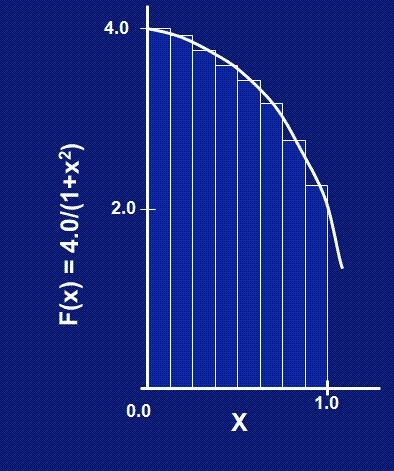
\includegraphics[width=4cm]{./pi}
    \end{center}
  \end{columns}

  \begin{algorithm}[H]
    \caption{Pseudo Code for Calculating Pi}
    \begin{algorithmic}
        \Function{calculate\_pi}{}
        \State $step \gets 1/n$
        \State $sum \gets 0$
        \Do{$i \gets 0\cdots n$}
        \State $x \gets (i+0.5)*step; sum \gets sum + 4/(1+x^2)$
        \EndDo
        \State $pi \gets sum * step$
        \EndFunction
    \end{algorithmic}
  \end{algorithm}
  \framebreak
  \begin{columns}
    \column{0.45\textwidth}
    \begin{exampleblock}{}
      \lstinputlisting[basicstyle=\fontsize{3}{3.5}\selectfont\ttfamily,language=OmpFortran]{src/calc_pi/solution/pi_acc.f90}
    \end{exampleblock}
    \column{0.45\textwidth}
    \begin{exampleblock}{}
      \lstinputlisting[basicstyle=\fontsize{3}{3.5}\selectfont\ttfamily,language=OmpC]{src/calc_pi/solution/pi_acc.c}
    \end{exampleblock}
  \end{columns}
\end{frame}

\begin{frame}[allowframebreaks]{Exercise 3: Matrix Multiplication}
  \begin{itemize}
    \item Most Computational code involve matrix operations such as matrix multiplication.
    \item Consider a matrix {\bf C} which is a product of two matrices {\bf A} and {\bf B}:
    \item[] Element {\it i,j} of {\bf C} is the dot product of the $i^{th}$ row of {\bf A} and $j^{th}$ column of {\bf B}
    \item Write a MATMUL code to multiple two matrices.
  \end{itemize}
  \begin{center}
    \includegraphics[width=0.6\textwidth]{./matmul}
  \end{center}

  \begin{algorithm}[H]
    \caption{Pseudo Code for MATMUL}
    \begin{algorithmic}
      \Program{matmul}{}
      \State $m,n \gets$ some\,large\,number $\le 1000$
      \State Define $a_{mn}, b_{nm}, c_{mm}$
      \State $a_{ij} \gets i+j; b_{ij} \gets i-j; c_{ij} \gets 0$
      \Do{$i \gets 1\cdots m$}
      \Do{$j \gets 1\cdots m$}
      \State $c_{i,j} \gets \sum^{n}_{k=1} a_{i,k}*b_{k,j}$
      \EndDo
      \EndDo
      \EndProgram{matmul}
    \end{algorithmic}
  \end{algorithm}
  \framebreak
  \begin{columns}
    \column{0.44\textwidth}
    \vspace{-1cm}
    \begin{exampleblock}{}
      \vspace{-0.25cm}
      \lstinputlisting[basicstyle=\fontsize{3}{3.5}\selectfont\ttfamily,language=OmpFortran]{src/matmul/solution/matmul_acc.f90}
    \end{exampleblock}
    \column{0.44\textwidth}
    \vspace{-1cm}
    \begin{exampleblock}{}
      \vspace{-0.25cm}
      \lstinputlisting[basicstyle=\fontsize{3}{3.5}\selectfont\ttfamily,language=OmpC]{src/matmul/solution/matmul_acc.c}
    \end{exampleblock}
  \end{columns}

\end{frame}
\end{document}

